\documentclass{beamer}
\usepackage{ctex, hyperref}
\usepackage[T1]{fontenc}

% other packages
\usepackage{latexsym,amsmath,xcolor,multicol,booktabs,calligra}
\usepackage{graphicx,pstricks,listings,stackengine}

\author{雷翔麟}
\title{SPREADSHEETBENCH}
\institute{华中科技大学计算机科学与技术学院}
\date{2024年10月10日}
\usepackage{HUST}

% defs
\def\cmd#1{\texttt{\color{red}\footnotesize $\backslash$#1}}
\def\env#1{\texttt{\color{blue}\footnotesize #1}}
\definecolor{deepblue}{rgb}{0,0,0.5}
\definecolor{deepred}{rgb}{0.6,0,0}
\definecolor{deepgreen}{rgb}{0,0.5,0}
\definecolor{halfgray}{gray}{0.55}

\lstset{
    basicstyle=\ttfamily\small,
    keywordstyle=\bfseries\color{deepblue},
    emphstyle=\ttfamily\color{deepred},    % Custom highlighting style
    stringstyle=\color{deepgreen},
    numbers=left,
    numberstyle=\small\color{halfgray},
    rulesepcolor=\color{red!20!green!20!blue!20},
    frame=shadowbox,
}


\begin{document}

\kaishu
\begin{frame}
    \titlepage
    \begin{figure}[htpb]
        \begin{center}
            
\includegraphics[width=0.2\linewidth]{pic/HUST_LOGO.png}
        \end{center}
    \end{figure}
\end{frame}

\begin{frame}
    \tableofcontents[sectionstyle=show,subsectionstyle=show/shaded/hide,subsubsectionstyle=show/shaded/hide]
\end{frame}

\section{Ideas}

\begin{frame}
    \frametitle{Five Key Ideas}
    \begin{itemize}
        \item Collect high-quality \textbf{data} from real-world sources and select the questions by rigorous criteria
        \item Utilize GPT-4 to recreate a coherent \textbf{instruction}
        \item Categorize \textbf{answer positions} into sheet-level and cell-level
        \item Create multiple spreadsheets and develop multiple \textbf{test cases} for each instruction
        \item Use various methods to mitigate \textbf{data leakage}
    \end{itemize}
\end{frame}

\begin{frame}
    \centering
    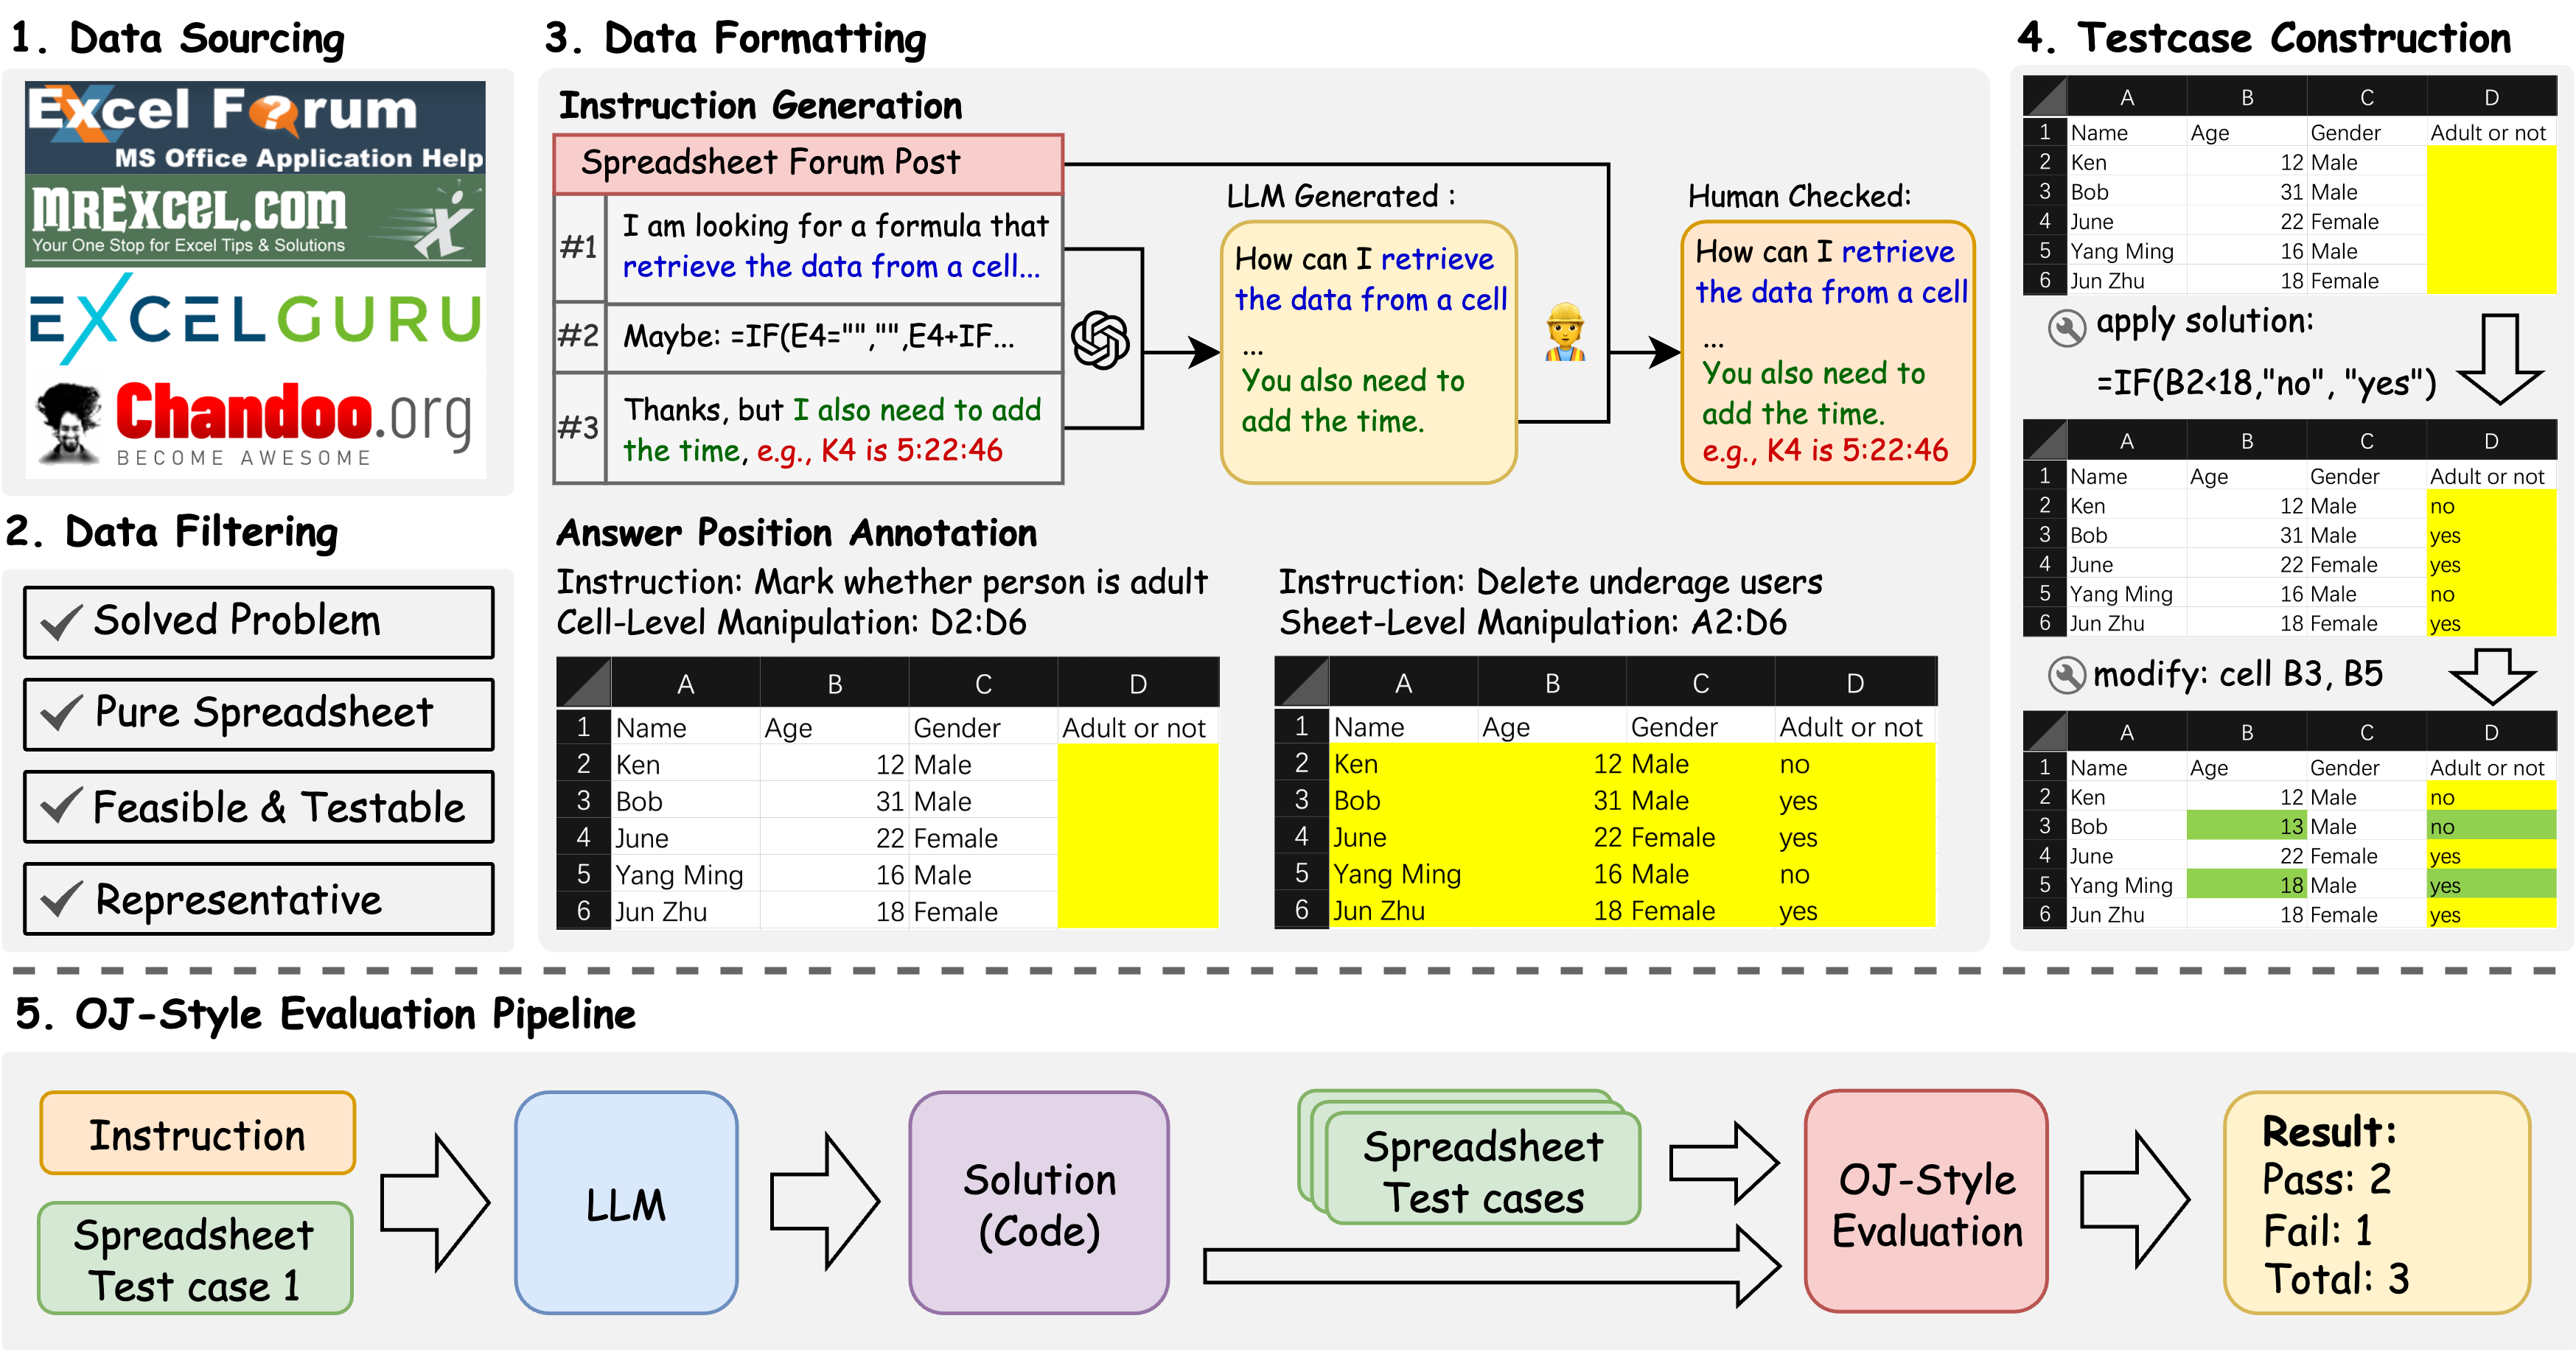
\includegraphics[width=1\linewidth]{pic/construction pipeline.png}
    \vspace{0.2cm}
    {\footnotesize Figure 1: The benchmark construction pipeline and OJ-style evaluation.}
\end{frame}

\section{Details}
\begin{frame}
    \frametitle{Data Info}
    \centering
    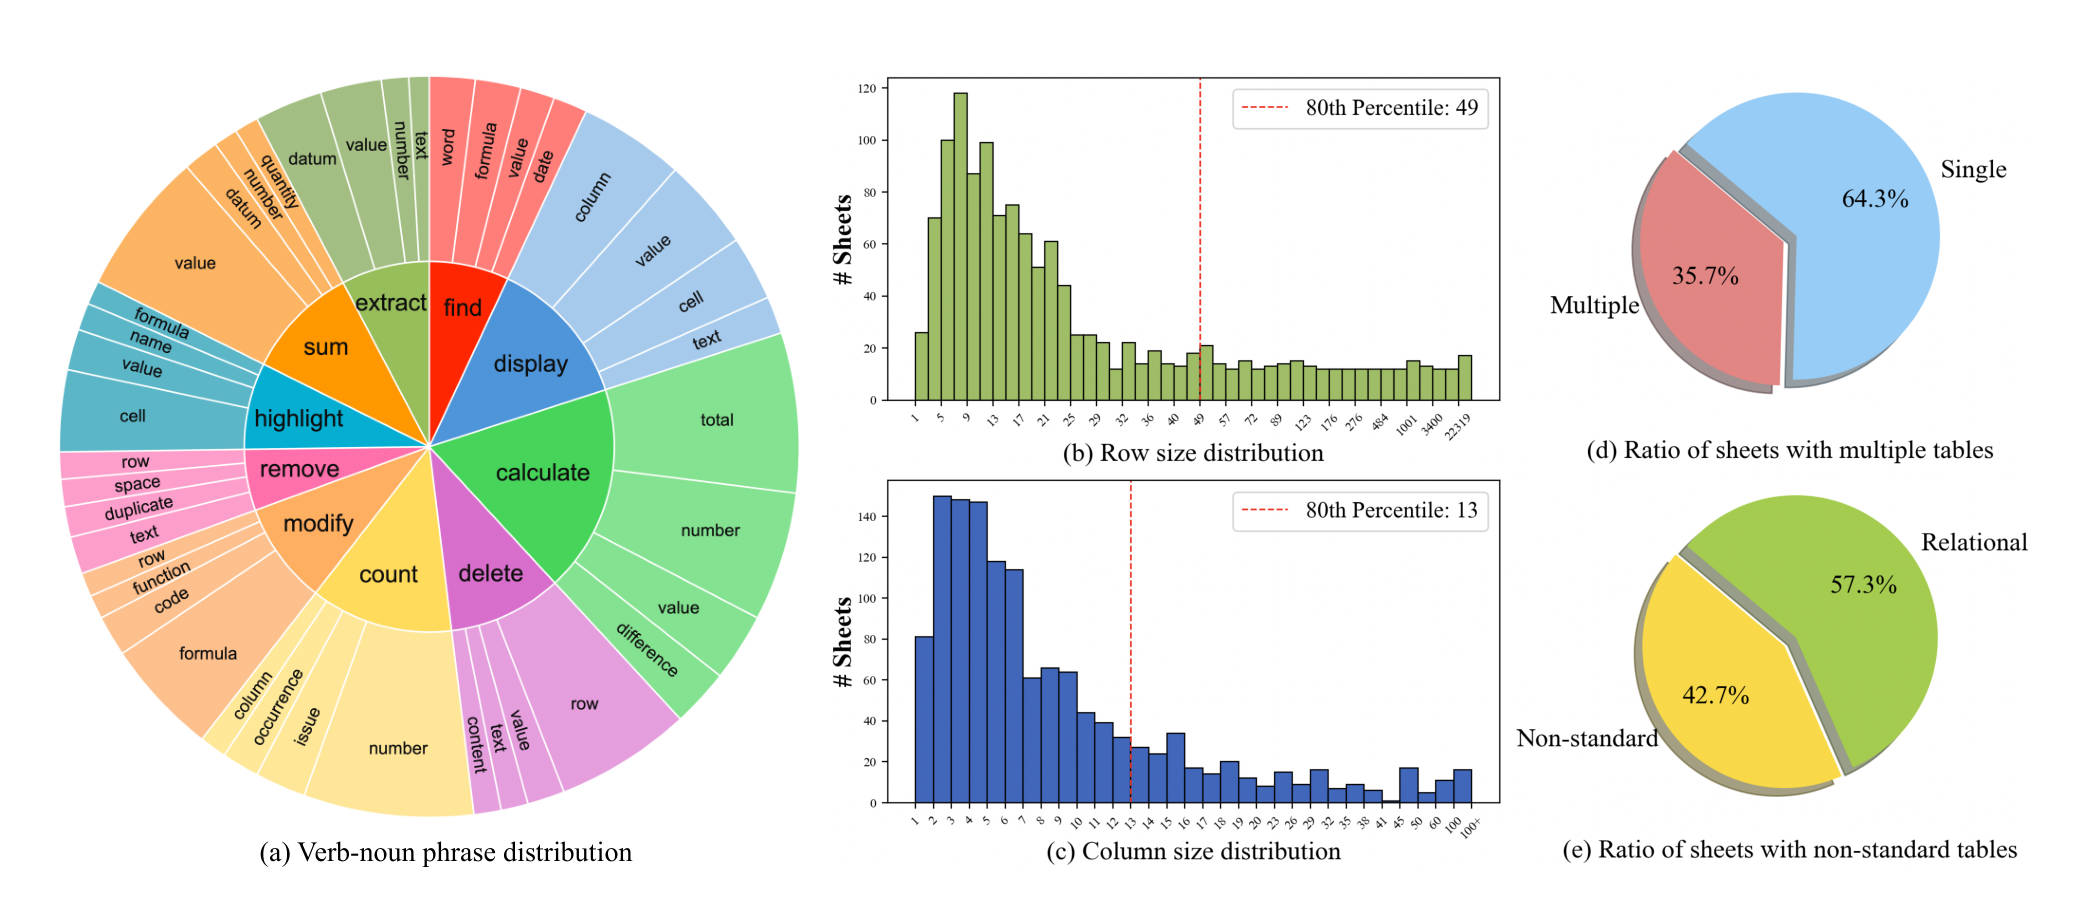
\includegraphics[width=1\linewidth]{pic/key statistics.jpg}
    \vspace{0.2cm}
    {\footnotesize Figure 2: Key statistics of SPREADSHEETBENCH.}
\end{frame}

\begin{frame}
    \frametitle{Data Leakage}
    \textbf{Issue:} Datasets initially \textbf{obtained from online} forums may be susceptible to data leakage issues, given that many LLMs are pre-trained using a vast corpus of web text.
    
    \textbf{Solutions:}
    \begin{itemize}
        \item \textbf{Revise the original questions} in the posts during the Instruction Generation process.
        \item \textbf{modifying the original provided spreadsheets} during the Spreadsheet Modification.
        \item \textbf{alter the position} of the tabular data in the original spreadsheets
        and the corresponding answer in the resulting spreadsheets during the Answer Position Changing
    \end{itemize}
\end{frame}

\begin{frame}
    \frametitle{Evaluation Metrics}
    \begin{itemize}
        \item \textbf{Soft Restriction:}
        $$ S _ { \text{soft} } = \frac { 1 } { | D | } \sum _ { i = 1 } ^ { | D | } \left( \frac { 1 } { | T _ { i } | } \sum _ { j = 1 } ^ { | T _ { i } | } 1 _ { r _ { i } = \text{ACC} } \right)$$

        \item \textbf{Hard Restriction:}
        $$ S _ { h a r d } = \frac { 1 } { | D | } \sum _ { i = 1 } ^ { | D | } 1 _ { r i j } = A C C , \forall j = 1 , 2 , \ldots , | T _ { i } |$$
    \end{itemize}
\end{frame}

\begin{frame}
    \frametitle{Inference Setting}
    Evaluate LLMs under two distinct settings:
    \begin{itemize}
        \item \textbf{Single-Round:} present the model with the initial few rows of spreadsheet files within the prompt, allowing for \textbf{only one inference}.
        \item \textbf{Multi-Round:} Building on the single-round prompt setting, furnish error feedback if the code fails to execute, enabling the model to refine its code in subsequent iterations.
    \end{itemize}
\end{frame}

\section{Codes}
\begin{frame}
    \frametitle{GitHub Link}
    GitHub Link: \href{https://github.com/RUCKBReasoning/SpreadsheetBench}{https://github.com/RUCKBReasoning/SpreadsheetBench}
\end{frame}

\section{Conclusion}
\begin{frame}
    \centering
    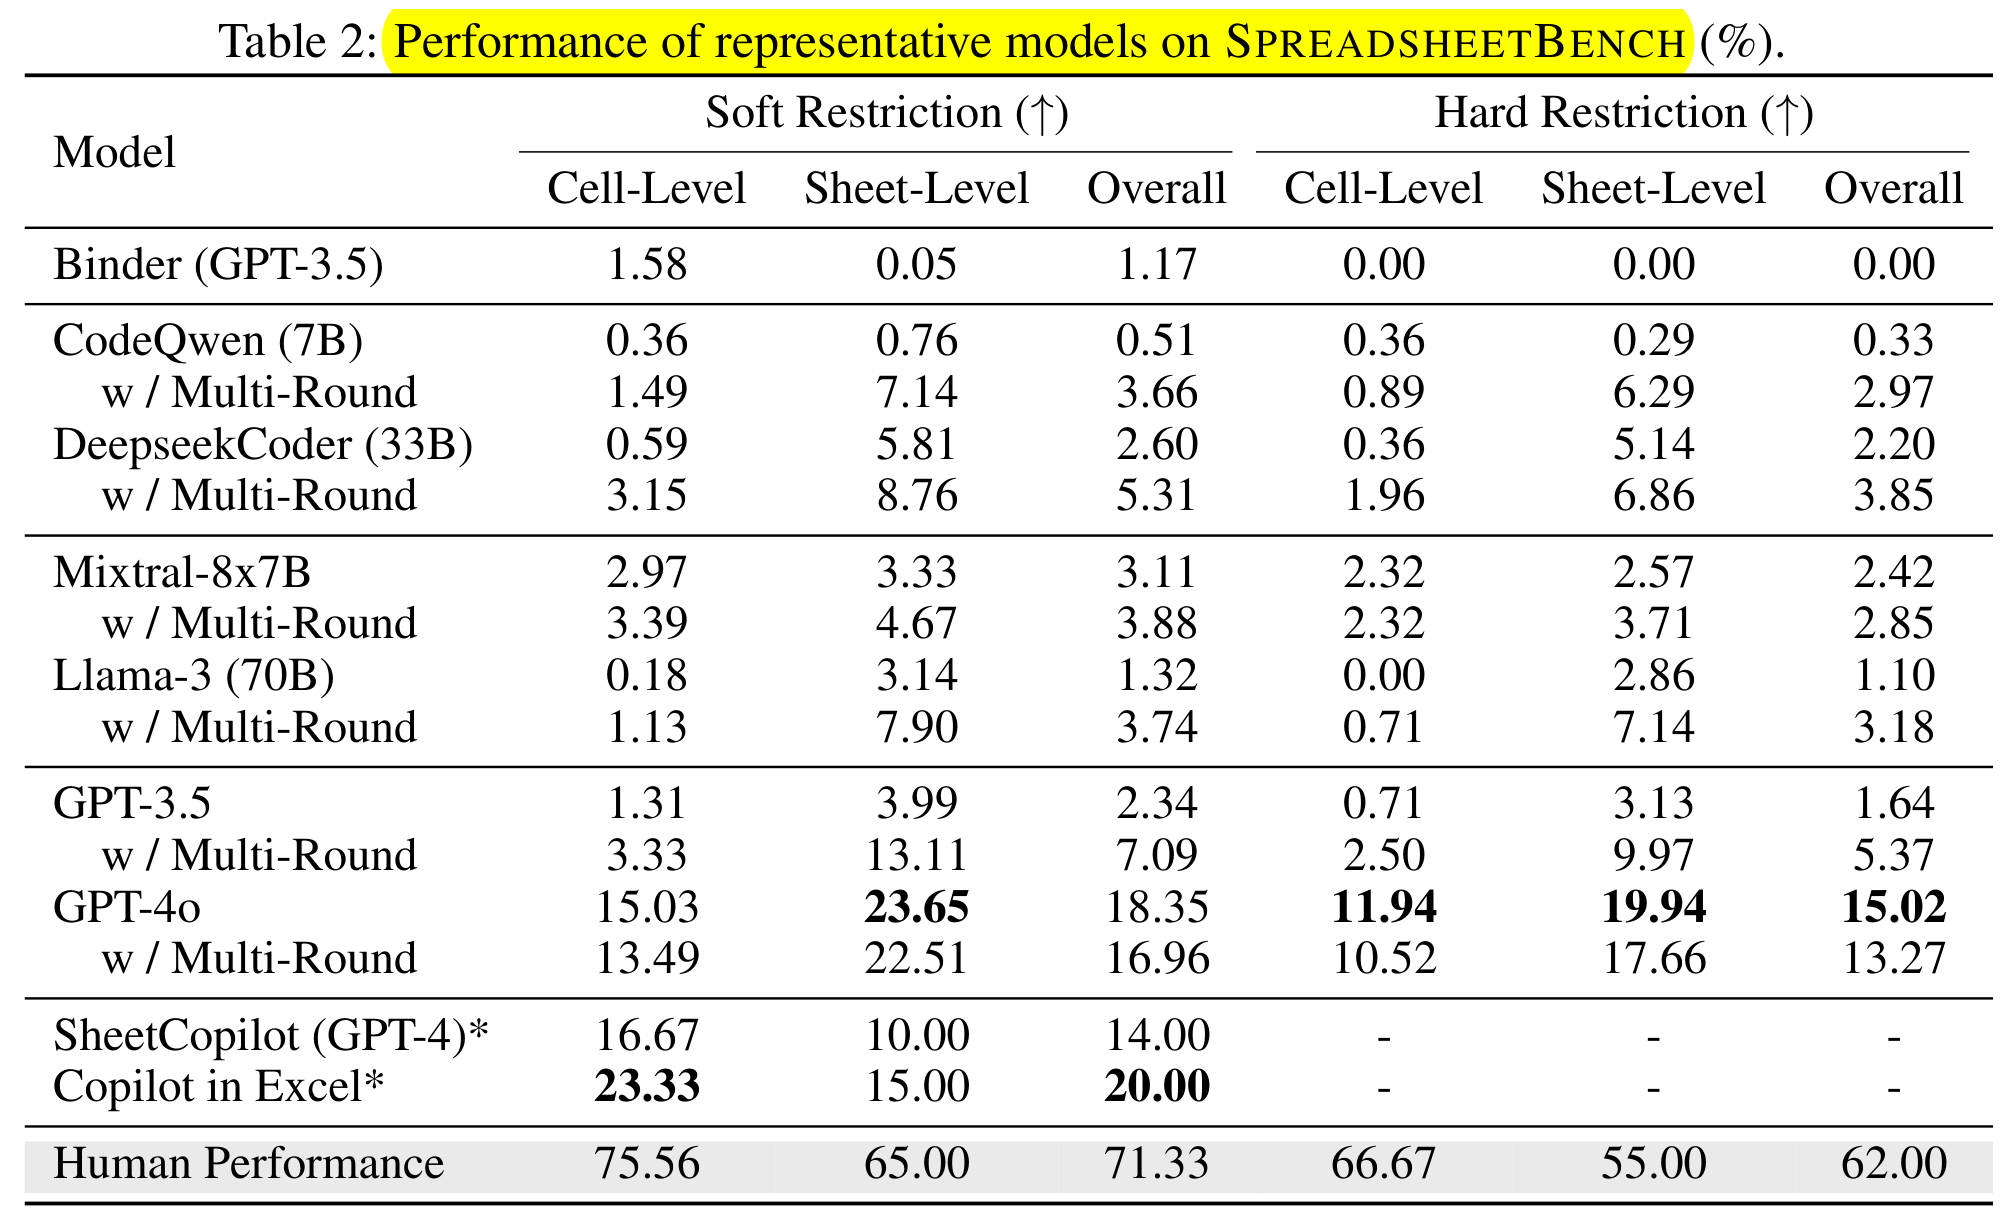
\includegraphics[width=1\linewidth]{pic/performance.jpg}
    \vspace{0.2cm}
    {\footnotesize Figure 3: Performance of representative models on SPREADSHEETBENCH \(\%\).}
\end{frame}

\section{Motivation}

\begin{frame}
    \begin{itemize}
        \item The concept of constructing a benchmark:
        \begin{itemize}
            \item Data quality
            \item Data construction
            \item Data diversity
        \end{itemize}
        \item Methods to address data leakage issues
        \item Developing a pipeline for evaluating problems using LLMs
        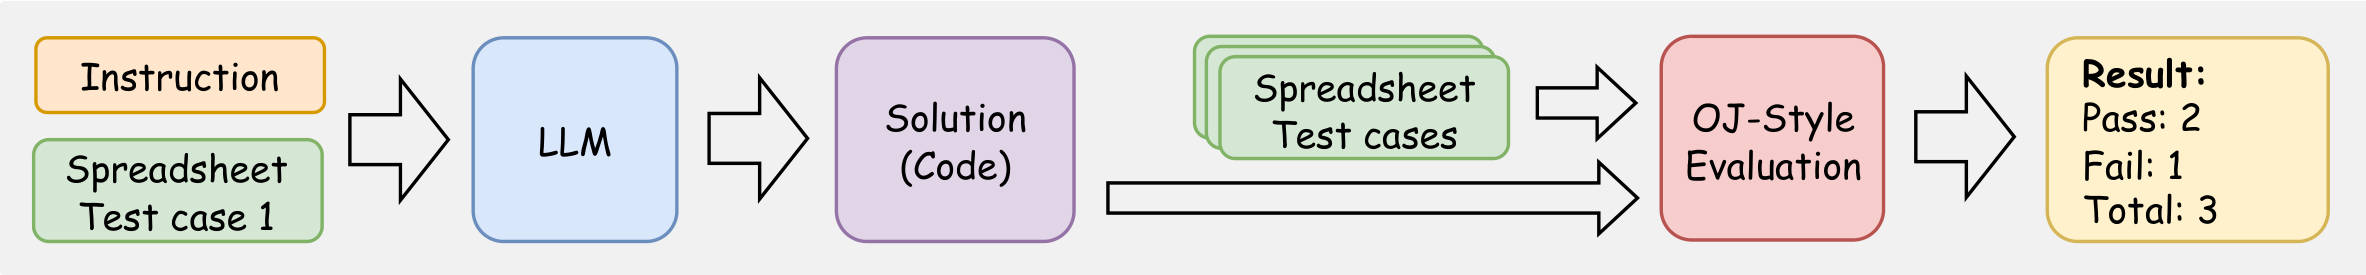
\includegraphics[width=1\linewidth]{pic/OJ Evaluation pipeline.jpg}
    \end{itemize}
\end{frame}

\begin{frame}
    \begin{center}
        {\Huge\calligra Thanks!}
    \end{center}
\end{frame}

\end{document}